\documentclass[tikz, border=12pt]{standalone}
\usepackage{tikz}
\usepackage{amsmath}
\usetikzlibrary{arrows.meta, positioning, calc, shapes.geometric}

% ==============================================================================
% SECTION 7 FSM - SYNCHRONIZED ACADEMIC PALETTE:
% Rich Deepened "Batata" (#FEF08A) Fills + Crisp Solid Black 2.4pt Borders
% Solid High-Visibility Signal Badges Matching Section 5 Datapath
% Continuous Solid Vectors for Write-Shortcut & Tree-PLRU Updates (Zero Dashes)
% ==============================================================================
\definecolor{fsmBatata}{HTML}{F5BC01}         % Rich Deepened "Batata" Fill (#fef08a)
\definecolor{fsmBatataBorder}{HTML}{000000}   % Solid Black Outline

% Stage Border & Wire Colors matching Datapath
\definecolor{borderIdle}{HTML}{059669}        % Emerald Green (#059669)
\definecolor{borderStage1}{HTML}{0284C7}      % Datapath Stage 1 Blue (#0284c7)
\definecolor{borderTag}{HTML}{D97706}         % Datapath Stage 2 Amber (#d97706)
\definecolor{borderHit}{HTML}{047857}         % Datapath Hit Green (#047857)
\definecolor{borderDecomp}{HTML}{8A2BE2}      % Datapath Stage 3 Purple (#8a2be2)
\definecolor{borderMiss}{HTML}{700018}        % Datapath Miss Burgundy (#700018)
\definecolor{borderWrite}{HTML}{102C60}       % Datapath Memory Navy (#102c60)
\definecolor{borderPlru}{HTML}{D97706}        % Datapath Tree-PLRU Amber (#d97706)

% Text Colors
\definecolor{textDark}{HTML}{0F172A}          % Dark Slate Text (#0f172a)

% Wire Colors matching Section 5 Datapath
\definecolor{wireSlate}{HTML}{1E293B}         % Crisp Dark Slate (#1e293b)
\definecolor{wireBlue}{HTML}{0284C7}          % Blue
\definecolor{wireOrange}{HTML}{D97706}        % Orange
\definecolor{wireGreen}{HTML}{047857}         % Green
\definecolor{wirePurple}{HTML}{8A2BE2}        % Purple
\definecolor{wireRed}{HTML}{DC2626}           % Red (#dc2626)

\begin{document}
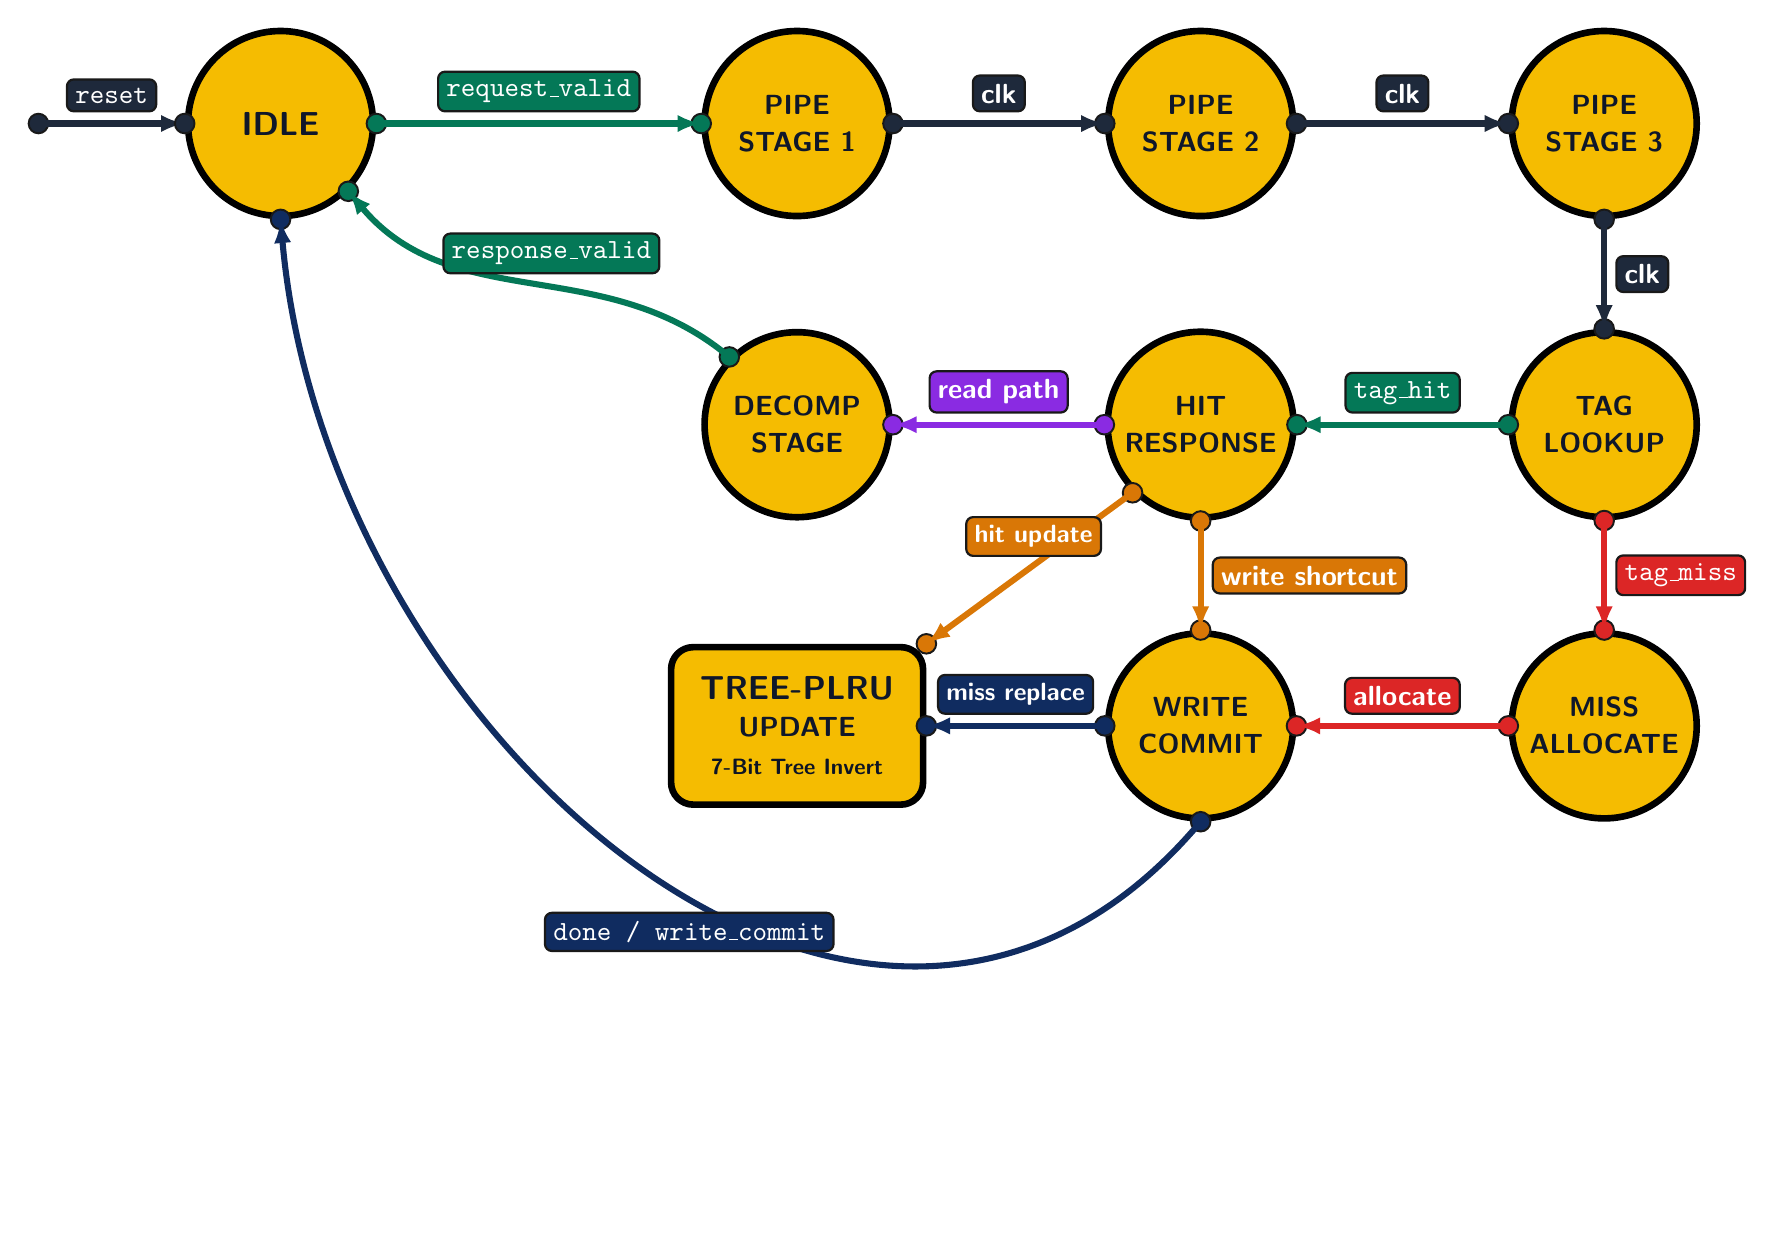
\begin{tikzpicture}[
    font=\sffamily,
    >=Latex,
    % "Batata" State Circles with Solid Crisp Black 2.4pt Borders
    stateNode/.style={circle, draw=black, fill=fsmBatata, line width=2.4pt,
                      minimum size=2.35cm, align=center, font=\sffamily\bfseries\normalsize, text=textDark},
    % Tree-PLRU Dedicated Hardware Unit Block (Matches State Colors & Borders)
    plruBlock/.style={rectangle, draw=black, fill=fsmBatata, line width=2.4pt, rounded corners=8pt,
                      minimum width=3.2cm, minimum height=2.0cm, align=center, text=textDark},
    % Terminal Pin Dot on Wire Ends
    pDot/.style={circle, fill=#1, inner sep=2.5pt, draw=black!90!white, line width=0.7pt},
    % Enlarged High-Visibility Signal Badges Matching Datapath (Solid Fill + Black Outline + White Text)
    badgeG/.style={fill=wireGreen, draw=black!90!white, line width=0.8pt, text=white, font=\sffamily\bfseries\normalsize, rounded corners=2.5pt, inner sep=3.0pt},
    badgeK/.style={fill=wireSlate, draw=black!90!white, line width=0.8pt, text=white, font=\sffamily\bfseries\normalsize, rounded corners=2.5pt, inner sep=3.0pt},
    badgeR/.style={fill=wireRed, draw=black!90!white, line width=0.8pt, text=white, font=\sffamily\bfseries\normalsize, rounded corners=2.5pt, inner sep=3.0pt},
    badgeP/.style={fill=wirePurple, draw=black!90!white, line width=0.8pt, text=white, font=\sffamily\bfseries\normalsize, rounded corners=2.5pt, inner sep=3.0pt},
    badgeO/.style={fill=wireOrange, draw=black!90!white, line width=0.8pt, text=white, font=\sffamily\bfseries\normalsize, rounded corners=2.5pt, inner sep=3.0pt},
    badgeN/.style={fill=borderWrite, draw=black!90!white, line width=0.8pt, text=white, font=\sffamily\bfseries\normalsize, rounded corners=2.5pt, inner sep=3.0pt},
    % Arrow Styles - All Continuous Solid Lines (Zero Dashes)
    wGreen/.style={->, line width=2.2pt, draw=wireGreen, >={Latex[length=3.0mm, width=2.2mm]}},
    wSlate/.style={->, line width=2.2pt, draw=wireSlate, >={Latex[length=3.0mm, width=2.2mm]}},
    wRed/.style={->, line width=2.2pt, draw=wireRed, >={Latex[length=3.0mm, width=2.2mm]}},
    wPurple/.style={->, line width=2.2pt, draw=wirePurple, >={Latex[length=3.0mm, width=2.2mm]}},
    wOrange/.style={->, line width=2.2pt, draw=wireOrange, >={Latex[length=3.0mm, width=2.2mm]}},
    wNavy/.style={->, line width=2.2pt, draw=borderWrite, >={Latex[length=3.0mm, width=2.2mm]}},
    x=4.1cm, y=2.25cm
]

%% ---- Row 1: IDLE and Stage 1 Pipeline (y = 0) ----
\node[stateNode] (IDLE)  at (-0.4, 0)  {\large IDLE};
\node[stateNode] (P1)    at (1.20, 0)  {PIPE\\[0.3ex]STAGE 1};
\node[stateNode] (P2)    at (2.45, 0)  {PIPE\\[0.3ex]STAGE 2};
\node[stateNode] (P3)    at (3.70, 0)  {PIPE\\[0.3ex]STAGE 3};

%% ---- Row 2: Tag Lookup, Hit Response & Decompressor (Shifted Down to y = -1.70) ----
\node[stateNode] (TLOOK)  at (3.70, -1.70)  {TAG\\[0.3ex]LOOKUP};
\node[stateNode] (HITR)   at (2.45, -1.70)  {HIT\\[0.3ex]RESPONSE};
\node[stateNode] (DECOMP) at (1.20, -1.70)  {DECOMP\\[0.3ex]STAGE};

%% ---- Row 3: Miss Allocate, Write Commit & Tree-PLRU Unit (y = -3.40) ----
\node[stateNode] (MALLOC) at (3.70, -3.40)  {MISS\\[0.3ex]ALLOCATE};
\node[stateNode] (WCOM)   at (2.45, -3.40)  {WRITE\\[0.3ex]COMMIT};

%% Tree-PLRU Dedicated Hardware Block (Balances 3x3 Grid Symmetrically!)
\node[plruBlock] (PLRU) at (1.20, -3.40) {
    {\large\textbf{TREE-PLRU}}\\[0.3ex]
    {\normalsize\textbf{UPDATE}}\\[0.4ex]
    {\footnotesize\textcolor{textDark!85!black}{\textbf{7-Bit Tree Invert}}}
};

%% ---- Entry RESET Arrow into IDLE ----
\node[pDot=wireSlate] at (-1.15, 0) {};
\draw[wSlate] (-1.15, 0) -- 
  node[above=4pt, badgeK]{\texttt{reset}} (IDLE.west);
\node[pDot=wireSlate] at (IDLE.west) {};

%% ---- Main Pipeline Path Arrows & Pin Dots ----
% IDLE -> P1 (request_valid - Green)
\node[pDot=wireGreen] at (IDLE.east) {};
\node[pDot=wireGreen] at (P1.west) {};
\draw[wGreen] (IDLE.east) -- 
  node[above=4pt, badgeG]{\texttt{request\_valid}} (P1.west);

% P1 -> P2 (clk - Slate)
\node[pDot=wireSlate] at (P1.east) {};
\node[pDot=wireSlate] at (P2.west) {};
\draw[wSlate] (P1.east) -- 
  node[above=4pt, badgeK]{\textit{clk}} (P2.west);

% P2 -> P3 (clk - Slate)
\node[pDot=wireSlate] at (P2.east) {};
\node[pDot=wireSlate] at (P3.west) {};
\draw[wSlate] (P2.east) -- 
  node[above=4pt, badgeK]{\textit{clk}} (P3.west);

% P3 -> TLOOK (clk - Slate)
\node[pDot=wireSlate] at (P3.south) {};
\node[pDot=wireSlate] at (TLOOK.north) {};
\draw[wSlate] (P3.south) -- 
  node[right=4pt, badgeK]{\textit{clk}} (TLOOK.north);

% TLOOK -> HITR (tag_hit - Green)
\node[pDot=wireGreen] at (TLOOK.west) {};
\node[pDot=wireGreen] at (HITR.east) {};
\draw[wGreen] (TLOOK.west) -- 
  node[above=4pt, badgeG]{\texttt{tag\_hit}} (HITR.east);

% TLOOK -> MALLOC (tag_miss - Red)
\node[pDot=wireRed] at (TLOOK.south) {};
\node[pDot=wireRed] at (MALLOC.north) {};
\draw[wRed] (TLOOK.south) -- 
  node[right=4pt, badgeR]{\texttt{tag\_miss}} (MALLOC.north);

% HITR -> DECOMP (read path - Purple)
\node[pDot=wirePurple] at (HITR.west) {};
\node[pDot=wirePurple] at (DECOMP.east) {};
\draw[wPurple] (HITR.west) -- 
  node[above=4pt, badgeP]{\textbf{read path}} (DECOMP.east);

% MALLOC -> WCOM (allocate - Red)
\node[pDot=wireRed] at (MALLOC.west) {};
\node[pDot=wireRed] at (WCOM.east) {};
\draw[wRed] (MALLOC.west) -- 
  node[above=4pt, badgeR]{\textbf{allocate}} (WCOM.east);

%% ---- Return Paths to IDLE ----
% DECOMP -> IDLE (response_valid - Green)
\node[pDot=wireGreen] at (DECOMP.north west) {};
\node[pDot=wireGreen] at (IDLE.south east) {};
\draw[wGreen] (DECOMP.north west) to[out=140, in=-50] (IDLE.south east);
\path (DECOMP.north west) to[out=140, in=-50] 
  node[pos=0.45, above=4pt, badgeG] {\texttt{response\_valid}} (IDLE.south east);

% WCOM -> IDLE (done / write_commit - Navy) - Sweeps generously underneath with zero overlap!
\node[pDot=borderWrite] at (WCOM.south) {};
\node[pDot=borderWrite] at (IDLE.south) {};
\draw[wNavy] (WCOM.south) to[out=-130, in=-85, looseness=1.20] (IDLE.south);
\path (WCOM.south) to[out=-130, in=-85, looseness=1.20] 
  node[pos=0.45, below=5pt, badgeN] {\texttt{done / write\_commit}} (IDLE.south);

%% ---- Write-Hit Shortcut (HITR -> WCOM - SOLID CONTINUOUS ORANGE VECTOR, NO DASHES!) ----
\node[pDot=wireOrange] at (HITR.south) {};
\node[pDot=wireOrange] at (WCOM.north) {};
\draw[wOrange] (HITR.south) -- 
  node[right=4pt, badgeO]{\textbf{write shortcut}} (WCOM.north);

%% ---- Solid Concurrent Updates to Tree-PLRU Block (CONTINUOUS SOLID VECTORS, NO DASHES!) ----
% 1. From HIT RESPONSE -> PLRU (Solid Orange Vector with Pin Dots)
\node[pDot=wireOrange] at (HITR.south west) {};
\node[pDot=wireOrange] at (PLRU.north east) {};
\draw[wOrange] (HITR.south west) -- 
  node[pos=0.48, above=3pt, badgeO, font=\sffamily\bfseries\small]{\textbf{hit update}} (PLRU.north east);

% 2. From WRITE COMMIT -> PLRU (Solid Navy Vector with Pin Dots)
\node[pDot=borderWrite] at (WCOM.west) {};
\node[pDot=borderWrite] at (PLRU.east) {};
\draw[wNavy] (WCOM.west) -- 
  node[above=4pt, badgeN, font=\sffamily\bfseries\small]{\textbf{miss replace}} (PLRU.east);

\end{tikzpicture}
\end{document}